\documentclass[10pt]{article}
\usepackage[margin=0.75in]{geometry}
\usepackage{amsmath,amssymb,booktabs,longtable,graphicx,xcolor,microtype}
\usepackage{xurl}
\usepackage[hidelinks]{hyperref}
\newcommand{\code}[1]{\texttt{#1}}
\title{Controlled-integrator remeasurement of the three-mode relaxation rates}
\author{Numerical audit report}
\date{7 September 2026}

\begin{document}
\maketitle

\section*{Verdict}

The controlled Cartesian calculation removes every suspected numerical feature
of the historical action--angle implementation: the state is double precision,
the timestep is fixed, standard mathematical functions are used, and there is
no positive-action projection or action floor.  Nevertheless, the frozen
common-plateau gate fails for both bath conditions at both timesteps.  Therefore
the accessible data do \emph{not} resolve a unique spectral gap.  Under the
predeclared interpretation gate, the observable dependence is retained as a
property of the accessible dynamics (multiple modes have not separated by the
latest statistically supported lags), rather than classified as a projection
artefact or a timestep-limited result.

This is a negative but sharper conclusion.  The resolved action-sector rates
are stable under timestep reduction, and the oscillatory mode in
$I_1-I_3$ survives with frequency near the historical value $5.35$.  What is
not supported is replacing the observable-specific decay rates by one common
number and calling that number the spectral gap.

\section{Frozen design and controlled dynamics}

The model has $n=3$, $\gamma=0.1$, burn-in 500, stationary measurement time
1000, snapshot interval 0.01, and 64 independent seeded trajectories.  Both
$(T_1,T_3)=(2,8)$ and $(5,5)$ were run at $\Delta t=10^{-3}$ and
$2.5\times10^{-4}$.  The full protocol, including all fit and interpretation
gates, was frozen before production.

The controlled state is $c_j=x_j+iy_j$ with $I_j=|c_j|^2$ and $E=H/2$.
Interior dynamics is $dc_j=i\nabla_jE\,dt$; each boundary obeys
\[
dc_r=(i-\gamma)\nabla_rE\,dt+\sqrt{2\gamma T_r}\,dW_r.
\]
Every fixed step uses an implicit-midpoint Hamiltonian update and Cartesian
Euler--Maruyama bath updates, with alternating bath order.  This is the same
projection-free representation used by the validated entropy sampler.  The
simulated state is float64; the twelve measured observables are stored as
float32.  The maximum arithmetic discrepancy in the stored sum/difference
identities was $8.94\times10^{-8}$.

\section{Frozen plateau results}

Figure~\ref{fig:rates} shows the local five-point log derivatives and
trajectory-bootstrap bands.  Thick segments mark plateaus accepted by the
frozen rule.  Table~\ref{tab:allrates} gives every requested observable,
including unresolved outcomes.

\begin{figure}[t]
\centering
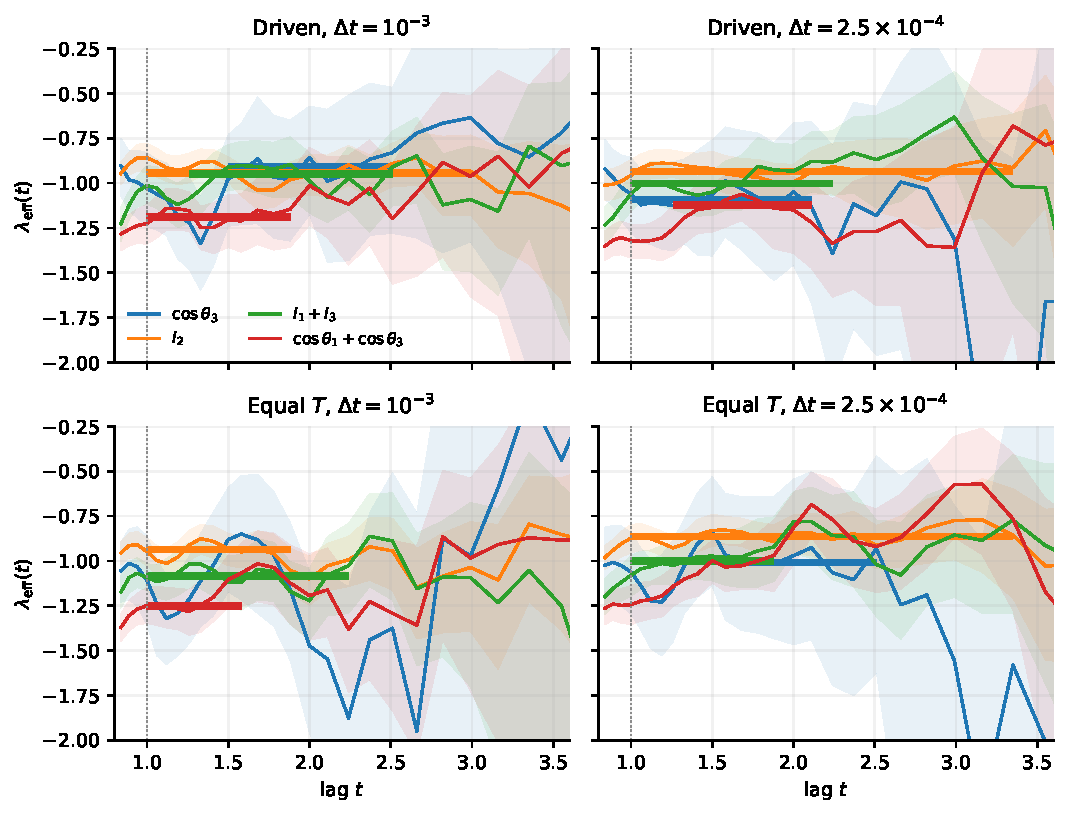
\includegraphics[width=\textwidth]{../figures/controlled_local_rates.pdf}
\caption{Controlled local decay rates.  Bands are trajectory-bootstrap 95\%
intervals; thick horizontal segments are the weighted rates on intervals
accepted by the unchanged plateau rule.  Loss of support at later lags produces
the visible noisy excursions and is not used to select a rate.}
\label{fig:rates}
\end{figure}

\begin{longtable}{lllrr}
\caption{Frozen-rule plateau results for every saved observable.}\label{tab:allrates}\\
\toprule Case & Observable & Window & $\widehat\lambda_R$ [95\% CI] & $N_{\rm eff}$ \\
\midrule\endfirsthead
\toprule Case & Observable & Window & $\widehat\lambda_R$ [95\% CI] & $N_{\rm eff}$ \\
\midrule\endhead
driven, $10^{-3}$ & $\cos\theta_1$ & -- & \multicolumn{1}{c}{UNRESOLVED} & 108664 \\
driven, $10^{-3}$ & $\sin\theta_1$ & -- & \multicolumn{1}{c}{UNRESOLVED} & 279157 \\
driven, $10^{-3}$ & $\cos\theta_3$ & [1.50,2.51] & -0.9080 [-1.1010,-0.7094] & 121229 \\
driven, $10^{-3}$ & $\sin\theta_3$ & -- & \multicolumn{1}{c}{UNRESOLVED} & 376027 \\
driven, $10^{-3}$ & $\cos(\theta_1-\theta_3)$ & -- & \multicolumn{1}{c}{UNRESOLVED} & 235152 \\
driven, $10^{-3}$ & $I_2$ & [1.00,2.99] & -0.9440 [-0.9906,-0.8998] & 54093 \\
driven, $10^{-3}$ & $I_1+I_3$ & [1.26,2.51] & -0.9491 [-1.0380,-0.8622] & 73980 \\
driven, $10^{-3}$ & $I_1-I_3$ & -- & \multicolumn{1}{c}{UNRESOLVED} & 173306 \\
driven, $10^{-3}$ & $\cos\theta_1+\cos\theta_3$ & [1.00,1.88] & -1.1878 [-1.2911,-1.0932] & 79710 \\
driven, $10^{-3}$ & $\cos\theta_1-\cos\theta_3$ & -- & \multicolumn{1}{c}{UNRESOLVED} & 218429 \\
driven, $10^{-3}$ & $\sin\theta_1+\sin\theta_3$ & -- & \multicolumn{1}{c}{UNRESOLVED} & 395151 \\
driven, $10^{-3}$ & $\sin\theta_1-\sin\theta_3$ & -- & \multicolumn{1}{c}{UNRESOLVED} & 248210 \\
\addlinespace
driven, $2.5\!\times\!10^{-4}$ & $\cos\theta_1$ & -- & \multicolumn{1}{c}{UNRESOLVED} & 105896 \\
driven, $2.5\!\times\!10^{-4}$ & $\sin\theta_1$ & -- & \multicolumn{1}{c}{UNRESOLVED} & 278826 \\
driven, $2.5\!\times\!10^{-4}$ & $\cos\theta_3$ & [1.00,2.11] & -1.0921 [-1.2129,-0.9686] & 126945 \\
driven, $2.5\!\times\!10^{-4}$ & $\sin\theta_3$ & -- & \multicolumn{1}{c}{UNRESOLVED} & 376126 \\
driven, $2.5\!\times\!10^{-4}$ & $\cos(\theta_1-\theta_3)$ & -- & \multicolumn{1}{c}{UNRESOLVED} & 245876 \\
driven, $2.5\!\times\!10^{-4}$ & $I_2$ & [1.00,3.35] & -0.9351 [-0.9975,-0.8697] & 55731 \\
driven, $2.5\!\times\!10^{-4}$ & $I_1+I_3$ & [1.00,2.24] & -1.0028 [-1.0768,-0.9364] & 74422 \\
driven, $2.5\!\times\!10^{-4}$ & $I_1-I_3$ & -- & \multicolumn{1}{c}{UNRESOLVED} & 174139 \\
driven, $2.5\!\times\!10^{-4}$ & $\cos\theta_1+\cos\theta_3$ & [1.26,2.11] & -1.1218 [-1.2439,-1.0146] & 79169 \\
driven, $2.5\!\times\!10^{-4}$ & $\cos\theta_1-\cos\theta_3$ & -- & \multicolumn{1}{c}{UNRESOLVED} & 218106 \\
driven, $2.5\!\times\!10^{-4}$ & $\sin\theta_1+\sin\theta_3$ & -- & \multicolumn{1}{c}{UNRESOLVED} & 394433 \\
driven, $2.5\!\times\!10^{-4}$ & $\sin\theta_1-\sin\theta_3$ & -- & \multicolumn{1}{c}{UNRESOLVED} & 248685 \\
\addlinespace
equal $T$, $10^{-3}$ & $\cos\theta_1$ & -- & \multicolumn{1}{c}{UNRESOLVED} & 122635 \\
equal $T$, $10^{-3}$ & $\sin\theta_1$ & -- & \multicolumn{1}{c}{UNRESOLVED} & 332646 \\
equal $T$, $10^{-3}$ & $\cos\theta_3$ & -- & \multicolumn{1}{c}{UNRESOLVED} & 121227 \\
equal $T$, $10^{-3}$ & $\sin\theta_3$ & -- & \multicolumn{1}{c}{UNRESOLVED} & 331774 \\
equal $T$, $10^{-3}$ & $\cos(\theta_1-\theta_3)$ & -- & \multicolumn{1}{c}{UNRESOLVED} & 242084 \\
equal $T$, $10^{-3}$ & $I_2$ & [1.00,1.88] & -0.9360 [-0.9930,-0.8836] & 57028 \\
equal $T$, $10^{-3}$ & $I_1+I_3$ & [1.00,2.24] & -1.0841 [-1.1670,-0.9997] & 78670 \\
equal $T$, $10^{-3}$ & $I_1-I_3$ & -- & \multicolumn{1}{c}{UNRESOLVED} & 177461 \\
equal $T$, $10^{-3}$ & $\cos\theta_1+\cos\theta_3$ & [1.00,1.58] & -1.2501 [-1.3545,-1.1521] & 83954 \\
equal $T$, $10^{-3}$ & $\cos\theta_1-\cos\theta_3$ & -- & \multicolumn{1}{c}{UNRESOLVED} & 224467 \\
equal $T$, $10^{-3}$ & $\sin\theta_1+\sin\theta_3$ & -- & \multicolumn{1}{c}{UNRESOLVED} & 403043 \\
equal $T$, $10^{-3}$ & $\sin\theta_1-\sin\theta_3$ & -- & \multicolumn{1}{c}{UNRESOLVED} & 257101 \\
\addlinespace
equal $T$, $2.5\!\times\!10^{-4}$ & $\cos\theta_1$ & -- & \multicolumn{1}{c}{UNRESOLVED} & 117212 \\
equal $T$, $2.5\!\times\!10^{-4}$ & $\sin\theta_1$ & -- & \multicolumn{1}{c}{UNRESOLVED} & 333400 \\
equal $T$, $2.5\!\times\!10^{-4}$ & $\cos\theta_3$ & [1.58,2.51] & -1.0081 [-1.3236,-0.7251] & 119815 \\
equal $T$, $2.5\!\times\!10^{-4}$ & $\sin\theta_3$ & -- & \multicolumn{1}{c}{UNRESOLVED} & 332753 \\
equal $T$, $2.5\!\times\!10^{-4}$ & $\cos(\theta_1-\theta_3)$ & -- & \multicolumn{1}{c}{UNRESOLVED} & 234498 \\
equal $T$, $2.5\!\times\!10^{-4}$ & $I_2$ & [1.00,3.35] & -0.8627 [-0.9165,-0.8119] & 53438 \\
equal $T$, $2.5\!\times\!10^{-4}$ & $I_1+I_3$ & [1.00,1.88] & -1.0010 [-1.0629,-0.9466] & 75878 \\
equal $T$, $2.5\!\times\!10^{-4}$ & $I_1-I_3$ & -- & \multicolumn{1}{c}{UNRESOLVED} & 177353 \\
equal $T$, $2.5\!\times\!10^{-4}$ & $\cos\theta_1+\cos\theta_3$ & -- & \multicolumn{1}{c}{UNRESOLVED} & 80196 \\
equal $T$, $2.5\!\times\!10^{-4}$ & $\cos\theta_1-\cos\theta_3$ & -- & \multicolumn{1}{c}{UNRESOLVED} & 224573 \\
equal $T$, $2.5\!\times\!10^{-4}$ & $\sin\theta_1+\sin\theta_3$ & -- & \multicolumn{1}{c}{UNRESOLVED} & 403883 \\
equal $T$, $2.5\!\times\!10^{-4}$ & $\sin\theta_1-\sin\theta_3$ & -- & \multicolumn{1}{c}{UNRESOLVED} & 256738 \\
\addlinespace
\bottomrule\end{longtable}
\begin{table}[t]\centering\small
\caption{Pooled common-plateau gate.  The eligible column lists observables that individually passed the frozen plateau rule.}\label{tab:common}
\begin{tabular}{lp{4.1cm}ccc}\toprule Case & Eligible & Spread pass & CI intersection & Verdict\\\midrule
driven, $10^{-3}$ & $\cos\theta_3$, $I_2$, $I_1+I_3$, $\cos\theta_1+\cos\theta_3$ & no & no & NO COMMON PLATEAU \\
driven, $2.5\!\times\!10^{-4}$ & $\cos\theta_3$, $I_2$, $I_1+I_3$, $\cos\theta_1+\cos\theta_3$ & yes & no & NO COMMON PLATEAU \\
equal $T$, $10^{-3}$ & $I_2$, $I_1+I_3$, $\cos\theta_1+\cos\theta_3$ & no & no & NO COMMON PLATEAU \\
equal $T$, $2.5\!\times\!10^{-4}$ & $\cos\theta_3$, $I_2$, $I_1+I_3$ & yes & no & NO COMMON PLATEAU \\
\bottomrule\end{tabular}\end{table}
\begin{longtable}{llll}
\caption{Historical versus controlled rates. Blank numerical entries mean the observable was unresolved; $\dagger$ means it was not saved historically.}\label{tab:comparison}\\
\toprule Bath & Observable & Historical & Controlled: $10^{-3}$; $2.5\times10^{-4}$\\\midrule\endfirsthead
\toprule Bath & Observable & Historical & Controlled: $10^{-3}$; $2.5\times10^{-4}$\\\midrule\endhead
driven & $\cos\theta_1$ & UNRESOLVED & UNRESOLVED; UNRESOLVED \\
driven & $\sin\theta_1$ & UNRESOLVED & UNRESOLVED; UNRESOLVED \\
driven & $\cos\theta_3$ & UNRESOLVED & -0.9080 [-1.1010,-0.7094]; -1.0921 [-1.2129,-0.9686] \\
driven & $\sin\theta_3$ & not saved$^\dagger$ & UNRESOLVED; UNRESOLVED \\
driven & $\cos(\theta_1-\theta_3)$ & UNRESOLVED & UNRESOLVED; UNRESOLVED \\
driven & $I_2$ & -0.9926 [-1.0517,-0.9337] & -0.9440 [-0.9906,-0.8998]; -0.9351 [-0.9975,-0.8697] \\
driven & $I_1+I_3$ & -1.1088 [-1.2013,-1.0228] & -0.9491 [-1.0380,-0.8622]; -1.0028 [-1.0768,-0.9364] \\
driven & $I_1-I_3$ & UNRESOLVED & UNRESOLVED; UNRESOLVED \\
equilibrium & $\cos\theta_1$ & -1.1878 [-1.3607,-1.0160] & UNRESOLVED; UNRESOLVED \\
equilibrium & $\sin\theta_1$ & UNRESOLVED & UNRESOLVED; UNRESOLVED \\
equilibrium & $\cos\theta_3$ & -1.1334 [-1.3366,-0.9465] & UNRESOLVED; -1.0081 [-1.3236,-0.7251] \\
equilibrium & $\sin\theta_3$ & not saved$^\dagger$ & UNRESOLVED; UNRESOLVED \\
equilibrium & $\cos(\theta_1-\theta_3)$ & UNRESOLVED & UNRESOLVED; UNRESOLVED \\
equilibrium & $I_2$ & -0.9065 [-0.9665,-0.8442] & -0.9360 [-0.9930,-0.8836]; -0.8627 [-0.9165,-0.8119] \\
equilibrium & $I_1+I_3$ & UNRESOLVED & -1.0841 [-1.1670,-0.9997]; -1.0010 [-1.0629,-0.9466] \\
equilibrium & $I_1-I_3$ & UNRESOLVED & UNRESOLVED; UNRESOLVED \\
\bottomrule\end{longtable}
\begin{longtable}{lllrrrl}
\caption{Predeclared early-window damped fits, all using $t\in[0.05,1.00]$.}\label{tab:odd}\\
\toprule Case & Observable & $\lambda_R$ [95\% CI] & $\lambda_I$ & 95\% CI & Period & $\Delta$AIC\\\midrule\endfirsthead
\toprule Case & Observable & $\lambda_R$ [95\% CI] & $\lambda_I$ & 95\% CI & Period & $\Delta$AIC\\\midrule\endhead
driven, $10^{-3}$ & $I_1-I_3$ & -5.0244 [-5.2494,-4.8249] & 5.4009 & [5.2495,5.5404] & 1.163 & -522.3 \\
driven, $10^{-3}$ & $\cos\theta_1-\cos\theta_3$ & -6.6106 [-7.0738,-6.1611] & 3.6464 & [3.4687,3.7771] & 1.723 & -299.1 \\
driven, $10^{-3}$ & $\sin\theta_1-\sin\theta_3$ & -3.3903 [-3.4321,-3.3471] & 4.0007 & [3.9091,4.0916] & 1.571 & -728.9 \\
driven, $2.5\!\times\!10^{-4}$ & $I_1-I_3$ & -5.0030 [-5.2637,-4.7820] & 5.4997 & [5.3420,5.6486] & 1.142 & -515.6 \\
driven, $2.5\!\times\!10^{-4}$ & $\cos\theta_1-\cos\theta_3$ & -6.3392 [-6.9625,-5.8337] & 3.3184 & [3.0874,3.4924] & 1.893 & -327.1 \\
driven, $2.5\!\times\!10^{-4}$ & $\sin\theta_1-\sin\theta_3$ & -3.3971 [-3.4383,-3.3584] & 4.0075 & [3.9186,4.0991] & 1.568 & -689.5 \\
equal $T$, $10^{-3}$ & $I_1-I_3$ & -4.1409 [-4.2475,-4.0436] & 5.0810 & [4.9343,5.2284] & 1.237 & -688.1 \\
equal $T$, $10^{-3}$ & $\cos\theta_1-\cos\theta_3$ & -5.4500 [-5.7716,-5.1626] & 3.4098 & [3.1736,3.6265] & 1.843 & -390.0 \\
equal $T$, $10^{-3}$ & $\sin\theta_1-\sin\theta_3$ & -3.5275 [-3.5792,-3.4764] & 4.3691 & [4.2719,4.4675] & 1.438 & -703.7 \\
equal $T$, $2.5\!\times\!10^{-4}$ & $I_1-I_3$ & -4.1845 [-4.3260,-4.0580] & 5.2637 & [5.1306,5.3869] & 1.194 & -878.1 \\
equal $T$, $2.5\!\times\!10^{-4}$ & $\cos\theta_1-\cos\theta_3$ & -5.5695 [-5.9128,-5.2754] & 3.4752 & [3.2296,3.6941] & 1.808 & -344.5 \\
equal $T$, $2.5\!\times\!10^{-4}$ & $\sin\theta_1-\sin\theta_3$ & -3.5204 [-3.5634,-3.4736] & 4.4719 & [4.3728,4.5701] & 1.405 & -709.4 \\
\bottomrule\end{longtable}
\begin{table}[t]\centering\small
\caption{Run-level numerical and stationarity audit.  $N_{\rm eff,last}$ is the smallest effective count among accepted plateaus after accounting for the terminal plateau lag.}\label{tab:audit}
\begin{tabular}{lrrrrr}\toprule Case & Proj./floor & Midpoint fail & Nonfinite & Worst burn-in metric & $N_{\rm eff,last}$\\\midrule
driven, $10^{-3}$ & 0/0 & 0 & 0 & 0.00498 & 53931 \\
driven, $2.5\!\times\!10^{-4}$ & 0/0 & 0 & 0 & 0.00218 & 55544 \\
equal $T$, $10^{-3}$ & 0/0 & 0 & 0 & 0.00180 & 56921 \\
equal $T$, $2.5\!\times\!10^{-4}$ & 0/0 & 0 & 0 & 0.00310 & 53259 \\
\bottomrule\end{tabular}\end{table}


The most favorable pooled case is the driven fine-timestep run: the four
resolved rates span $-1.122$ to $-0.935$, which passes the 20\% spread test, but
their 95\% intervals have no common intersection.  The coarse driven run fails
both spread and CI intersection.  At equal temperature the pooled and exact
exchange-even sector tests also fail.  No exchange-odd observable has a late
positive-correlation plateau under the frozen $t\ge1$ rule.

\section{Timestep control and comparison with the inherited integrator}

Where both controlled timesteps resolve an observable, the estimates are
timestep-consistent by the predeclared CI-overlap plus 20\% rule.  In the driven
case the relative changes are 18.4\% for $\cos\theta_3$, 0.94\% for $I_2$, and
5.51\% for $I_1+I_3$.  At equal temperature they are 8.15\% for $I_2$ and
7.97\% for $I_1+I_3$.  Thus there is no pattern in which the common plateau
appears only at the finer step; the result is not classified as
timestep-limited.

The action-sector values remain close to the inherited calculation.  For
example, driven $I_2$ changes from $-0.993$ historically to $-0.944$ and
$-0.935$, while driven $I_1+I_3$ changes from $-1.109$ to $-0.949$ and
$-1.003$.  Their uncertainty intervals overlap or nearly overlap.  Removing
the projection therefore changes details but does not create a common
observable-independent asymptotic window.

\section{Exchange combinations and oscillatory modes}

The exact endpoint-exchange combinations could not be formed in the historical
run because $\sin\theta_3$ was absent.  Here both sine endpoints were saved.
At equilibrium, sums are exchange-even and differences are exchange-odd; in
the driven case these names only identify the same coordinates because the
baths break exchange symmetry.

All predeclared early-window damped fits strongly beat the nested real
exponential (Table~\ref{tab:odd}; every $\Delta$AIC is below $-299$), and all
2000 bootstrap replicates succeeded.  The $I_1-I_3$ frequencies are 5.401 and
5.500 in the driven runs and 5.081 and 5.264 in equilibrium.  Their intervals
are compatible across the two timesteps and with the historical estimate
$5.35$ (period $1.174$).  Hence that particular complex-mode frequency is
confirmed.

The other exact odd combinations do not share the same frequency:
$\cos\theta_1-\cos\theta_3$ gives approximately 3.3--3.6 and
$\sin\theta_1-\sin\theta_3$ gives approximately 4.0--4.5.  Thus the odd sector
contains more than one visible damped mode in the predeclared early window; the
value 5.35 is not a universal odd-sector eigenfrequency.

\begin{figure}[t]
\centering
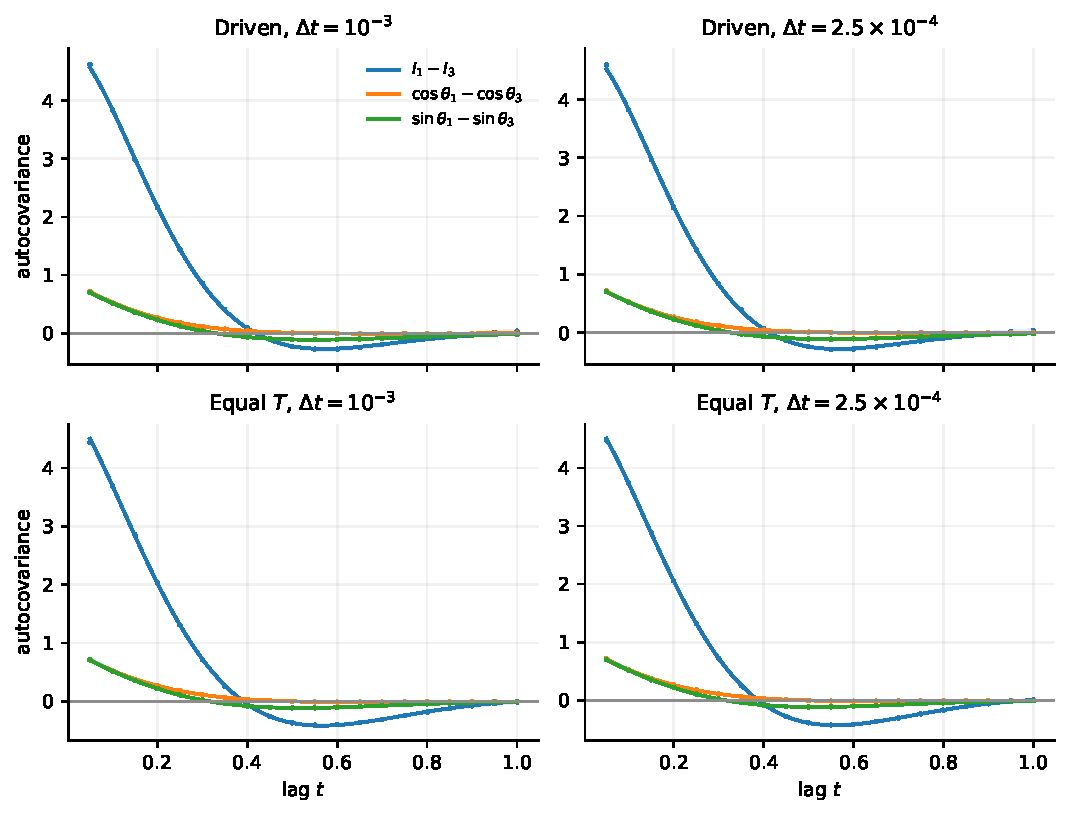
\includegraphics[width=\textwidth]{../figures/controlled_odd_damped_fits.pdf}
\caption{Direct autocovariances (points and one-standard-error bands) and
predeclared damped-oscillation fits (lines) on $t\in[0.05,1.00]$.}
\label{fig:odd}
\end{figure}

\section{Numerical integrity, burn-in, and effective support}

Each run contains exactly 64 streams and 100001 snapshots per stream.  Every
saved value is finite.  Across all four runs the projection count, floor count,
zero-radius count, midpoint-failure count, and nonfinite count are all zero.
The minimum sampled actions range from $1.17\times10^{-8}$ to
$1.64\times10^{-7}$, so the controlled calculation directly samples the
near-zero-action region without clipping it.

The unchanged discard-first-quarter burn-in metric passes for every observable
in every run; its worst value is 0.00498, an order of magnitude below the 0.05
gate.  The smallest effective count at the terminal lag of any accepted
plateau is 53259.  Statistical support is therefore substantial, although it
still ends before a common asymptotic mode separates.

\section{Provenance and reproducibility}

The frozen remote commit is
\nolinkurl{fddd8c5a1700675a702aadab5dac9262ab48f6c6}; the equivalent local launch
commit is \nolinkurl{899a5d345a98e4c8d5605a6a5a166a08bb86adcd}.
The production source SHA-256 is
\nolinkurl{58c871882f1180701a7aae637a8f4be113315a72fb9d7815562f5fc90faf7976};
the binary SHA-256 is
\nolinkurl{f7cd820bb8f716a8790f688db060259da5657e4f20fa09100546e66efb696b3f}.
Production ran from 17:45:09 to 17:47:23 UTC on 7 September 2026.

The base seeds are 2026090801, 2026090802, 2026090803, and 2026090804 in the
matrix order stated above; all 64 realized stream seeds are recorded in each
\nolinkurl{metadata.csv}.  Exact commands are recorded in
\nolinkurl{provenance/production_commands.txt}.  The integrity audit and
SHA-256 of every raw stream are in
\nolinkurl{provenance/integrity_audit.json} and
\nolinkurl{provenance/raw_artifact_manifest.sha256}.

\section*{Claim boundary}

Supported: projection-free, fixed-step controlled dynamics yields stable
observable-specific decay rates; the driven action observables decay near
$-0.94$ to $-1.00$ in the accepted windows; and the $I_1-I_3$ complex mode has
frequency near 5.35.  Not supported: a common late-time rate across the
requested observables, a unique numerical spectral gap, or identification of
all exchange-odd probes with a single complex eigenpair.

\end{document}
